\chapter{State of the art} \label{}


Some 1986's Dawkins's research was the pioneer of a significant addition to the
1990s IEC algorithms research works\cite{dawkins1986blind}[Dawkins 1986].

There is two key research approach about his field:

Creative Approach: The Artificial Life (AL) was the base of creative approach.
AL uses complex algorithms for biological life models emulation. To perform this
task, it is needed to include some of the different techniques starting from
right image treatment. Good graphic creation as well as a great music and
quality sounds, \cite{sims1991artificial}[Sims 1991b], \cite{sims1994evolving}[Sims 1994],
\cite{dawkins1986blind}[Dawkins 1986], \cite{disz1997ubiworld}[Disz 1997],
\cite{unemi2000sbart}[Unemi 2000]and \cite{unemi2003sbeat3}[Unemi
2003].
 
Humanized technology approach: The concept of humanized technology approach
comes from the approach that is focused on the IEC algorithms interface, this is
the research of interaction between humans and computer systems. The main goal
of this was to reduce the user's fatigue and to promote the inputs and outputs
of algorithms to improve the efficiency of them. IEC has made his own way in
practical fields such as engineering, education,etc.,
\cite{parmee1993concrete}[Parmee 1993], \cite{ventrella1994explorations}[Ventrella 1994a],
\cite{takagi1996discrete}[Takagi 1996], \cite{poli1997genetic}[Poli 1997],
\cite{parmee1998genetic}[Parmee 1998] and \cite{takagi1998interactive}[Takagi 1998].

Computer graphics (CG) The Biomorph of Dawkins was the first IEC research, from
this research comes to many motivated works mostly about the Selfish Gene, come
of these works are:  \cite{ochoa1998genetic}[Ochoa 1998],
\cite{mccormack1993interactive}[Mccormack 1993], and
\cite{}[Smith 2003].

In Dawkins work, a conventional recursive algorithm was used as a baseline
maintaining the main target of trees with an L-system (Lindenmayer). This same
L-system was the base for another experiment to create 2-D CG forms insects from
a system called Blind Watchmaker who used L-system angles from L-system output
intuitively selected; the creation was called biomorphs. These creations reach
his target with the multiple selections of the users based on their preferences;
all these selections acted like a natural adaptation filter.

We can find plenty of applications and works for fractal generation [Sims 1991a]
and \cite{sims1992interactive}[Sims 1992], \cite{baluja1993simulating}[Baluja
1993] and \cite{baluja1994towards}[Baluja 1994], \cite{lund1995artistic}[Lund
1995], or \cite{angeline1996evolving}[Angeline
1996],\cite{raynal1999manipulation}[Raynal 1999] and
\cite{lutton2003artie}[Lutton 2003], for rendering in tridimensional,
\cite{todd1992artificial}[Todd 1991],\cite{broughton1997use}[Broughton 1997],
\cite{das1994genetic}[Das 1994] and \cite{tam2002genetic}[Tam 2002], for
generation of virtual creatures, \cite{}[Sims 1994],
\cite{rowland2000evolutionary}[Rowland 2000], or aerodynamic surface design
(wings), \cite{nguyen1993evolvable}[NGuyen 1993],
\cite{nguyen1994evolvable}[NGuyen 1994] and \cite{}[NGuyen 1997].

We can discover more than one additional way to use this research in the
artistic field with several applications of IEC who are used for cartoon face
construction and animations matters, like Mutator \cite{}[Todd 1991], \cite{todd1994evolutionary}[Todd 1994]
and \cite{todd1999mutation}[Todd 1999] or \cite{bentley1999introduction}[Bentley 1999a].

The genetic programming (GP) applications offers a category called Interactive
Genetic Programming (IGP) with many examples of successful application in
tridimensional artwork for artistic animations or construction using
mathematical equations as CAVE \cite{das1994genetic}[Das 1994],
\cite{papka1996ubiworld}[Papka 1996] and \cite{disz1997ubiworld}[Disz 1997],
\cite{}[Sims 1991], \cite{sims1991artificial}[Sims 1991a],
\cite{sims1992interactive}[Sims 1992] and \cite{min2004creative}[Min 2004]. As
this work consequence, Panspermia or Primordial Dance was created that are
presented in figure \ref{fig:Panspermia} and figure \ref{fig:PrimordialD}.

\begin{figure*}
\captionsetup{justification=centering,margin=2cm}
\centering
\setlength\fboxsep{0pt}
\setlength\fboxrule{0.7pt}
\fbox{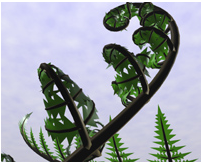
\includegraphics[width=10cm,height=10cm,keepaspectratio]{img/Panspermia.png}}
\caption{Panspermia.}
\label{fig:Panspermia}       
\end{figure*}

\begin{figure*}
\captionsetup{justification=centering,margin=2cm}
\centering
\setlength\fboxsep{0pt}
\setlength\fboxrule{0.7pt}
\fbox{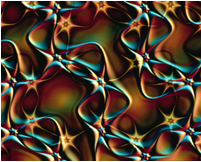
\includegraphics[width=10cm,height=10cm,keepaspectratio]{img/PrimordialDance.png}}
\caption{Primordial Dance.}
\label{fig:PrimordialD}       
\end{figure*}


The artistic field is only the first step of a great IEC implementation; it is
important to mention another relevant projects called Galapagos, \cite{sims1997interactivity}[Sims 1997],
and SBART, \cite{unemi2000sbart} [Unemi 2000]. The IEC application Galapagos Project is the exhibit in
Tokio Multimedia Museum, (NTT Intercommunication Center) and this project
originates engaging images to all visitors based on L-systems as we can see in figure \ref{fig:Galapagos1} 
and figure \ref{fig:Galapagos2}.

\begin{figure*}
\captionsetup{justification=centering,margin=2cm}
\centering
\setlength\fboxsep{0pt}
\setlength\fboxrule{0.7pt}
\fbox{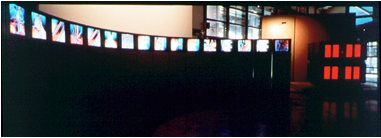
\includegraphics[width=10cm,height=10cm,keepaspectratio]{img/Galapagos1.png}}
\caption{Galapagos: Tokio Multimedia Museum.}
\label{fig:Galapagos1}       
\end{figure*}

\begin{figure*}
\captionsetup{justification=centering,margin=2cm}
\centering
\setlength\fboxsep{0pt}
\setlength\fboxrule{0.7pt}
\fbox{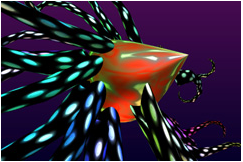
\includegraphics[width=10cm,height=10cm,keepaspectratio]{img/Galapagos2.png}}
\caption{Galapagos' output sample.}
\label{fig:Galapagos2}       
\end{figure*}

There are created after one selection, to get a good solution through multiple
repetitions. This action is performed with Genetic Programming (GP), after the
calculation of each pixel value using trees of equations combining logarithm,
maximum, and minimum, sine, root, cosine, exponential arithmetic operators.
AnimationLab is found as an outstanding work who offer figures that can run or
walk working with the user to receive more opportunities to be picked. A
particular characteristic of all of the figures is that the figures extremities
Mentioning open source works, we can find SBART as an IGP
\cite{unemi2000sbart}[Unemi 2000] tool to create graphics. SBART allow to users
to evaluate 20 two-dimensional images, subsequently twenty new image has
direction and angles as we can see in figure \ref{fig:AnimationLab}.

\begin{figure*}
\captionsetup{justification=centering,margin=2cm}
\centering
\setlength\fboxsep{0pt}
\setlength\fboxrule{0.7pt}
\fbox{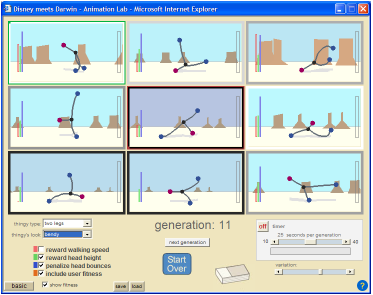
\includegraphics[width=10cm,height=10cm,keepaspectratio]{img/AnimationLab.png}}
\caption{Animation Lab.}
\label{fig:AnimationLab}       
\end{figure*}

There are many examples for this field application as
\cite{mckenna1990dynamic}[McKenna 1990],
\cite{ventrella1994explorations}[Ventrella 1994a], or
\cite{ventrella1995disney}[Ventrella 1995], \cite{lim1999pro}[Lim 1999] and
\cite{lim2000solve}[Lim 2000].  One of the Interactive Evolutionary Programming
(IEP)  artistic application was created by \cite{angeline1996evolving}[Angeline
1996], as a fractal generation where the system allows the evolution of
animations for the ones who were selected from the user, the application
initially show only 10 animations to rate.


It is important to know how IEC was implemented in music generation, with
several applications in this field. We will start mentioning the pioneer
application GENJAM, \cite{biles1994genjam}[Biles 1994],
\cite{biles1996neural}[Biles 1996] or \cite{biles1999life}[Biles 1999] and
\cite{biles2002genjam}[Biles 2000]. Some other attractive works are Sonomorph,
\cite{nelson1993sonomorphs}[Nelson 1993] and \cite{nelson1995further}[Nelson
1995], or SBEAT, \cite{unemi2003sbeat3}[Unemi 2003],
\cite{horowitz1994generating}[Horowitz 1994], \cite{onisawa2000composition}[Onisawa
2000], \cite{tokui2000music}[Tokui 2000] and
\cite{fels2002interactive}[Fels 2002]. It is possible to hear a part of the
music songs of these previously mentioned works broadcasted in the radio station
WDYN. (100.1, New York, USA, WEBPage:http://www.wdyn.net/).

The IEC algorithms are the base for the functionality of the music generation
systems, a visual representation of this is given in the below figure \ref{fig:GENJAM}:

\begin{figure*}
\captionsetup{justification=centering,margin=2cm}
\centering
\setlength\fboxsep{0pt}
\setlength\fboxrule{0.7pt}
\fbox{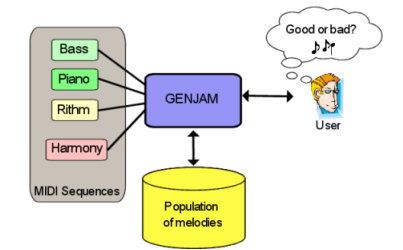
\includegraphics[width=10cm,height=10cm,keepaspectratio]{img/GENJAM.png}}
\caption{GENJAM squeme.}
\label{fig:GENJAM}       
\end{figure*}

In 1998, a new input method for human operators of an interactive genetic algo-
rithm to reduce the psychological weight is proposed. This method uses a
discrete fitness values to reduce the psychological stress involved in the input
procedure. They perform simulations to investigate the influence of the
resulting quantization noise from the use of discrete values of fitness in
convergence. Showing that the quantization noise does not significantly worsen
in the convergence. In this method they evaluated using two subjective tests
involving the task of drawing faces.

The subjective test results shows that this method significantly reduce the
level of psychological stress of human interactive genetic algorithms operators
\cite{ohsaki1998input}. Another approach, proposed to used novel method
evaluation. Where the user only evaluates a satisfactory or unsatisfactory
individual. These approach consider the level of sensibility of the different
users to their perception of the beautiful and the ugly, and fitness is
automatically calculated based on user evaluations and time. They also propose
effective strategies for comparing different individuals of the same generation
in uncertain fitness conditions of an individual. Where they obtains the
probability of an individual dominance by use of the probability of the interval
domain, and translate to a fuzzy number in a range based on α-cut set
\cite{gong2009impact}. They determine the dominant individual in tournament
selection with size being two on base given by the probability of a particular
domain. This approach was applied to an interactive evolutionary system for
fashion design. In figure 1 we can see dif-ferent user interfaces they used.
Based on this approach, another work was de-rived. Where the approach adopt a
fuzzy number described with a Gaussian mem-bership function to express an
individual's fitness. In order to compare the different individuals, they
generated a fitness interval based on a cut set, and ob-tain the probability of
interactive genetic algorithms with individual's fuzzy fitness. The
contributions in this approach can improve the performance of existing income
generating activities in alleviating user fatigue and finding optimal solutions
to an optimization problem, so it is beneficial for solving complicated problems
with implicit or fuzzy indices \cite{gong2011interactive} we can see the user
interface in figure \ref{fig:fashion}.

\begin{figure*}
\captionsetup{justification=centering,margin=2cm}
\centering
\setlength\fboxsep{0pt}
\setlength\fboxrule{0.7pt}
\fbox{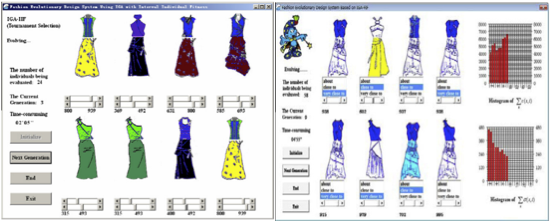
\includegraphics[width=10cm,height=10cm,keepaspectratio]{img/fashion.png}}
\caption{Different user interfaces interactive evolutionary system for fashion design.}
\label{fig:fashion}       
\end{figure*}

In Web-Based IEC aplications are two interesting works EndlessForms and Picbreeder.

Picbreeder is a Web-based application that allows users to evolve images in a
col-laborative way maintaining a large catalog of user-created content allowing
users collaboration by searching through extensive design spaces
\cite{secretan2008picbreeder}. Picbreeder provides to users of all
experience levels to enjoy all the creative contributions produced by other
users. In this way users experience a new form of recreation called creative
social recreation through collaborative exploration. In this sense these systems
helps their users to find interesting images through tagging, browsing and
searching as figure  \ref{fig:Picbreeder} show.

\begin{figure*}
\captionsetup{justification=centering,margin=2cm}
\centering
\setlength\fboxsep{0pt}
\setlength\fboxrule{0.7pt}
\fbox{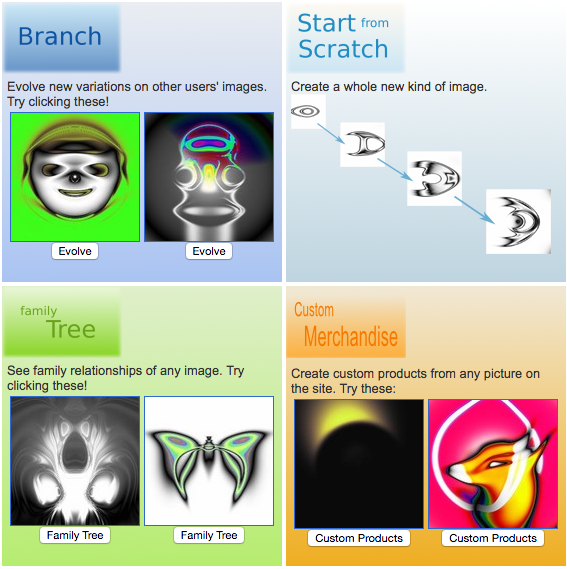
\includegraphics[width=10cm,height=10cm,keepaspectratio]{img/Picbreeder.png}}
\caption{Picbreeder User Selection.}
\label{fig:Picbreeder}       
\end{figure*}

EndlessForms is a Web application that Explore object designs by choosing those
the users like. These selected objects become the parents of the next generation
of objects \cite{clune2011evolving}. EndLessForms proposes a new way to evolve
3D objects inspired by biological morphologies using generative encoding. One of
the experiments proposed in this paper was to use interactive evolutionary
systems to determine the potential for generating complex and interesting 3D
objects. They chose the interactive evolution, because that allows openended
exploration of the design space of objects that can produce by their method.
Additionally, the interactive evolution avoids the greedy nature of evolution by
objectives, which potentially allows to access more interesting objects
\cite{clune2011evolving}. In figure \ref{fig:EndlessForms} we can see some of
this objects.

\begin{figure*}
\captionsetup{justification=centering,margin=2cm}
\centering
\setlength\fboxsep{0pt}
\setlength\fboxrule{0.7pt}
\fbox{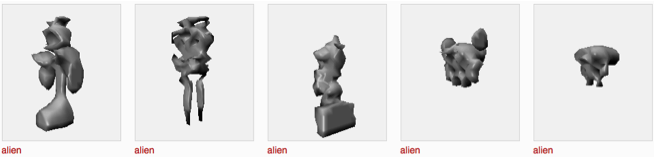
\includegraphics[width=10cm,height=10cm,keepaspectratio]{img/EndlessForms.png}}
\caption{Alien objects from EndLessForms.}
\label{fig:EndlessForms}       
\end{figure*}






